\clearpage
\cleardoublepage

\chapter{Transformer Architecture}

\section{Introduction}

The Transformer architecture, introduced by Vaswani et al.\ in 2017, fundamentally changed the landscape of sequence modeling and representation learning. By replacing recurrence with self-attention mechanisms, Transformers enable parallel computation across entire sequences, dramatically improving training efficiency and enabling the scaling to billions of parameters.

This chapter provides a comprehensive treatment of the Transformer architecture, from the fundamental attention mechanism to modern large language models.

\section{The Attention Mechanism}

\subsection{Background: RNN Limitations}

Before Transformers, sequence models relied on Recurrent Neural Networks (RNNs) and their variants (LSTM, GRU). While effective, RNNs suffer from:
\begin{itemize}
    \item \textbf{Sequential computation:} Cannot parallelize across time steps
    \item \textbf{Long-range dependencies:} Gradient propagation through many steps causes vanishing/exploding gradients
    \item \textbf{Computational inefficiency:} Each time step requires loading the hidden state from memory
\end{itemize}

\subsection{Scaled Dot-Product Attention}

The fundamental building block is the scaled dot-product attention:

\begin{equation}
\text{Attention}(\mathbf{Q}, \mathbf{K}, \mathbf{V}) = \text{softmax}\left(\frac{\mathbf{Q}\mathbf{K}^T}{\sqrt{d_k}}\right)\mathbf{V}
\label{eq:attention}
\end{equation}

where:
\begin{itemize}
    \item $\mathbf{Q} \in \mathbb{R}^{n \times d_k}$: Query matrix
    \item $\mathbf{K} \in \mathbb{R}^{m \times d_k}$: Key matrix
    \item $\mathbf{V} \in \mathbb{R}^{m \times d_v}$: Value matrix
    \item $d_k$: Dimension of keys (also query dimension)
\end{itemize}

\begin{note}[Why Scaled?]
The scaling factor $\sqrt{d_k}$ prevents the dot products from growing large in magnitude, which would push the softmax into regions with extremely small gradients. When $d_k$ is large, the dot products tend to be large, causing softmax to saturate (output close to one-hot).
\end{note}

\subsection{Self-Attention}

Self-attention is attention applied to a sequence where queries, keys, and values all come from the same source:

\begin{equation}
\mathbf{X}_{\text{out}} = \text{Attention}(\mathbf{X}\mathbf{W}_Q, \mathbf{X}\mathbf{W}_K, \mathbf{X}\mathbf{W}_V)
\end{equation}

where $\mathbf{W}_Q, \mathbf{W}_K, \mathbf{W}_V$ are learned projection matrices.

Key properties:
\begin{itemize}
    \item \textbf{All-to-all connections:} Each position can attend to all other positions
    \item \textbf{Constant path length:} Information flows in $O(1)$ steps regardless of distance
    \item \textbf{Computational complexity:} $O(n^2 \cdot d)$ for sequence length $n$ and dimension $d$
\end{itemize}

\section{Multi-Head Attention}

Rather than performing a single attention function, we project the queries, keys, and values $h$ times with learned linear projections:

\begin{equation}
\text{MultiHead}(\mathbf{Q}, \mathbf{K}, \mathbf{V}) = \text{Concat}\left(\text{head}_1, \ldots, \text{head}_h\right)\mathbf{W}^O
\end{equation}

where each head is:
\begin{equation}
\text{head}_i = \text{Attention}\left(\mathbf{Q}\mathbf{W}_i^Q, \mathbf{K}\mathbf{W}_i^K, \mathbf{V}\mathbf{W}_i^V\right)
\end{equation}

Typical configuration: $h = 8$ heads, $d_k = d_v = d_{\text{model}}/h$.

\begin{properties}[Multi-Head Attention Benefits]
\begin{itemize}
    \item Each head can attend to different aspects of the representation
    \item Different heads may specialize: positional, syntactic, semantic information
    \item The model can jointly attend to information from different representation subspaces
\end{itemize}
\end{properties}

\section{Transformer Architecture}

\subsection{Feed-Forward Networks}

Each layer includes a position-wise feed-forward network:
\begin{equation}
\text{FFN}(\mathbf{x}) = \mathbf{W}_2 \, \sigma\left(\mathbf{W}_1 \mathbf{x} + \mathbf{b}_1\right) + \mathbf{b}_2
\end{equation}

Typically implemented as two linear transformations with a ReLU activation. The inner dimension is usually $4 \times d_{\text{model}}$.

\subsection{Layer Normalization}

Layer normalization stabilizes training by normalizing activations:
\begin{equation}
\mathbf{y} = \frac{\mathbf{x} - \mu}{\sqrt{\sigma^2 + \epsilon}} \odot \gamma + \beta
\end{equation}
where $\mu = \frac{1}{d}\sum_{i=1}^d x_i$ and $\sigma^2 = \frac{1}{d}\sum_{i=1}^d (x_i - \mu)^2$.

Two variants exist:
\begin{itemize}
    \item \textbf{Post-LN (Original):} LayerNorm after residual connections
    \item \textbf{Pre-LN:} LayerNorm before attention/FFN (more stable for deep networks)
\end{itemize}

\subsection{Residual Connections}

Each sub-layer has a residual connection:
\begin{equation}
\mathbf{x}_{\text{out}} = \mathbf{x} + \text{SubLayer}(\mathbf{x})
\end{equation}

This enables gradient flow through skip connections and allows the network to learn identity mappings when beneficial.

\begin{figure}[htbp]
    \centering
    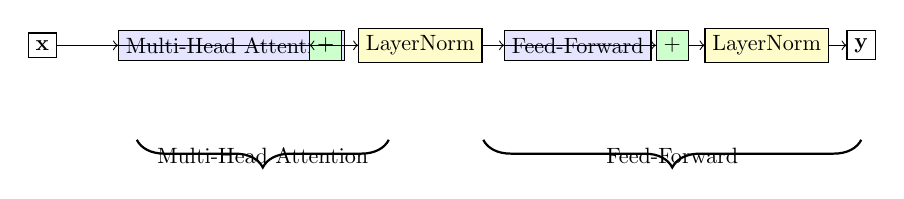
\begin{tikzpicture}[scale=0.8, every node/.style={scale=0.8}]
        % Input
        \node[draw, rectangle] (input) at (0, 0) {$\mathbf{x}$};
        
        % Multi-Head Attention
        \node[draw, rectangle, minimum width=2cm, fill=blue!10] (mha) at (3, 0) {Multi-Head Attention};
        \node[draw, rectangle, fill=green!20] (add1) at (4.5, 0) {$+$};
        \node[draw, rectangle, fill=yellow!20] (ln1) at (6, 0) {LayerNorm};
        
        % FFN
        \node[draw, rectangle, minimum width=2cm, fill=blue!10] (ffn) at (8.5, 0) {Feed-Forward};
        \node[draw, rectangle, fill=green!20] (add2) at (10, 0) {$+$};
        \node[draw, rectangle, fill=yellow!20] (ln2) at (11.5, 0) {LayerNorm};
        
        % Output
        \node[draw, rectangle] (output) at (13, 0) {$\mathbf{y}$};
        
        % Arrows
        \draw[->] (input) -- (mha);
        \draw[->] (mha) -- (add1);
        \draw[->] (add1) -- (ln1);
        \draw[->] (ln1) -- (ffn);
        \draw[->] (ffn) -- (add2);
        \draw[->] (add2) -- (ln2);
        \draw[->] (ln2) -- (output);
        
        % Skip connections
        \draw[-] (input) to[out=0, in=180] (add1);
        \draw[-] (ln1) to[out=0, in=180] (add2);
        
        % Bracket
        \draw[decorate, decoration={brace, amplitude=10pt, mirror}, thick] (1.5, -1.5) -- (5.5, -1.5) node[below, midway] {Multi-Head Attention};
        \draw[decorate, decoration={brace, amplitude=10pt, mirror}, thick] (7, -1.5) -- (13, -1.5) node[below, midway] {Feed-Forward};
    \end{tikzpicture}
    \caption{Transformer layer with residual connections and layer normalization.}
    \label{fig:transformer_layer}
\end{figure}

\section{Positional Encoding}

Since self-attention is permutation-invariant (invariant to input order), we must inject positional information:

\begin{equation}
\text{PE}_{(pos, 2i)} = \sin\left(\frac{pos}{10000^{2i/d_{\text{model}}}}\right)
\end{equation}
\begin{equation}
\text{PE}_{(pos, 2i+1)} = \cos\left(\frac{pos}{10000^{2i/d_{\text{model}}}}\right)
\end{equation}

where $pos$ is the position and $i$ is the dimension.

\begin{properties}[Positional Encoding Properties]
\begin{itemize}
    \item \textbf{Linear relationships:} $\text{PE}(pos+k)$ can be represented as a linear function of $\text{PE}(pos)$
    \item \textbf{Generalization:} Can encode positions beyond training sequence length
    \item \textbf{Relative positions:} Rotary Position Embedding (RoPE) encodes relative positions more directly
\end{itemize}
\end{properties}

Alternative: Rotary Position Embedding (RoPE) used in LLaMA and GPT-NeoX, which encodes relative position directly into the attention computation.

\section{Encoder-Decoder Architecture}

The original Transformer uses an encoder-decoder structure:

\begin{itemize}
    \item \textbf{Encoder:} $N$ identical layers processing the input sequence
    \item \textbf{Decoder:} $N$ identical layers with cross-attention to encoder outputs
    \item \textbf{Cross-attention:} Queries from decoder attend to keys/values from encoder
\end{itemize}

\begin{code}
    \captionof{listing}{PyTorch Multi-Head Attention Implementation}
    \label{code:mha_pytorch_ch12}
\begin{lstlisting}[language=python]
import torch
import torch.nn as nn
import torch.nn.functional as F
import math

class MultiHeadAttention(nn.Module):
    def __init__(self, d_model, num_heads):
        super().__init__()
        assert d_model % num_heads == 0
        
        self.d_model = d_model
        self.num_heads = num_heads
        self.d_k = d_model // num_heads
        
        self.W_q = nn.Linear(d_model, d_model)
        self.W_k = nn.Linear(d_model, d_model)
        self.W_v = nn.Linear(d_model, d_model)
        self.W_o = nn.Linear(d_model, d_model)
    
    def split_heads(self, x, batch_size):
        """Split the last dimension into num_heads."""
        x = x.view(batch_size, -1, self.num_heads, self.d_k)
        return x.permute(0, 2, 1, 3)  # (batch, heads, seq, d_k)
    
    def forward(self, query, key, value, mask=None):
        batch_size = query.size(0)
        
        # Linear projections
        Q = self.W_q(query)
        K = self.W_k(key)
        V = self.W_v(value)
        
        # Split heads
        Q = self.split_heads(Q, batch_size)
        K = self.split_heads(K, batch_size)
        V = self.split_heads(V, batch_size)
        
        # Scaled dot-product attention
        scores = torch.matmul(Q, K.transpose(-2, -1)) / math.sqrt(self.d_k)
        
        if mask is not None:
            scores = scores.masked_fill(mask == 0, -1e9)
        
        attention_weights = F.softmax(scores, dim=-1)
        attention_output = torch.matmul(attention_weights, V)
        
        # Concatenate heads
        attention_output = attention_output.permute(0, 2, 1, 3).contiguous()
        attention_output = attention_output.view(batch_size, -1, self.d_model)
        
        # Final linear projection
        output = self.W_o(attention_output)
        
        return output, attention_weights
\end{lstlisting}
\end{code}

\section{Vision Transformer (ViT)}

Vision Transformer applies the Transformer architecture to image classification by treating image patches as tokens:

\begin{enumerate}
    \item Split image into $16 \times 16$ patches
    \item Flatten each patch and project to $d_{\text{model}}$ dimensions
    \item Add [CLS] token (for classification) and positional embeddings
    \item Process through standard Transformer encoder
    \item Use [CLS] token output for classification
\end{enumerate}

Computational complexity: $O(n^2)$ where $n = \frac{H \times W}{P^2}$ is the number of patches.

\section{Large Language Models}

\subsection{GPT Architecture}

GPT (Generative Pre-trained Transformer) uses a decoder-only architecture:
\begin{itemize}
    \item Causal (masked) self-attention to prevent attending to future tokens
    \item Language modeling objective: predict next token
    \item Pre-training on large text corpus, then fine-tuning
\end{itemize}

GPT-3 scaled to 175 billion parameters, demonstrating emergent capabilities.

\subsection{BERT Architecture}

BERT uses an encoder-only architecture with bidirectional attention:
\begin{itemize}
    \item Masked Language Modeling (MLM): predict masked tokens
    \item Next Sentence Prediction (NSP): predict if one sentence follows another
    \item Enables deep bidirectional representations
\end{itemize}

\subsection{Modern LLMs}

Modern large language models incorporate several innovations:

\begin{table}[ht]
    \centering
    \caption{Comparison of Modern LLM Architectures}
    \begin{tabular}{L{2.5cm} L{3cm} L{3cm} L{3cm}}
        \toprule
        \textbf{Model} & \textbf{Architecture} & \textbf{Position Encoding} & \textbf{Key Features} \\
        \midrule
        GPT-2 & Decoder-only & Learned & Unigram tokenization \\
        GPT-3 & Decoder-only & Learned & In-context learning \\
        LLaMA & Decoder-only & RoPE & Efficient architecture \\
        ChatGLM & Prefix-LM & RoPE & Bilingual pre-training \\
        Mistral & Decoder-only & RoPE & Grouped-query attention \\
        \bottomrule
    \end{tabular}
\end{table}

Key architectural differences:
\begin{itemize}
    \item \textbf{RoPE (Rotary Position Embedding):} Encodes position in rotation matrix, better for relative positions
    \item \textbf{Grouped-Query Attention (GQA):} Multiple query heads share key/value heads, reduces memory
    \item \textbf{SwiGLU activation:} Used in LLaMA, better than GeGLU
    \item \textbf{Flash Attention:} IO-aware exact attention algorithm, reduces memory from $O(n^2)$ to $O(n)$
\end{itemize}

\section{Efficiency Considerations}

\subsection{Attention Complexity}

Standard attention has $O(n^2)$ complexity in sequence length, which becomes prohibitive for long sequences:

\begin{itemize}
    \item \textbf{Flash Attention:} Approximate attention with IO-awareness, 2-4x speedup
    \item \textbf{Sparse Attention:} Attend only to a subset of positions (Longformer, BigBird)
    \item \textbf{Linear Attention:} Kernel-based approximation with $O(n)$ complexity (Performer)
    \item \textbf{Low-rank attention:} Decompose attention matrix (Linformer)
\end{itemize}

\subsection{Memory Optimization}

For large models, memory becomes critical:
\begin{itemize}
    \item \textbf{Gradient checkpointing:} Trade compute for memory
    \item \textbf{Mixed precision:} FP16/BF16 training reduces memory by 2x
    \item \textbf{Quantization:} INT8/INT4 for inference
    \item \textbf{Paged attention:} Memory paging for KV cache (vLLM)
\end{itemize}

\section{Chapter Summary}

\begin{enumerate}
    \item Self-attention enables parallel computation and captures long-range dependencies with $O(1)$ path length
    \item Scaled dot-product attention with $\sqrt{d_k}$ scaling prevents gradient saturation
    \item Multi-head attention allows attending to different representation subspaces
    \item Residual connections and layer normalization enable stable training of deep networks
    \item Positional encoding injects order information since attention is permutation-invariant
    \item Vision Transformer (ViT) applies the Transformer architecture to images via patch embeddings
    \item Modern LLMs (GPT, BERT, LLaMA) scale Transformers to billions of parameters
    \item Efficiency techniques (Flash Attention, sparse attention, quantization) enable practical deployment of large models
\end{enumerate}

\section{Further Reading}

\begin{itemize}
    \item \cite{vaswani2017attention} --- Attention Is All You Need (Original Transformer paper)
    \item \cite{dosovitskiy2020image} --- An Image is Worth 16x16 Words: Transformers for Image Recognition at Scale (ViT)
    \item \cite{radford2019language} --- Language Models are Unsupervised Multitask Learners (GPT-2)
    \item \cite{brown2020language} --- Language Models are Few-Shot Learners (GPT-3)
    \item \cite{devlin2018bert} --- BERT: Pre-training of Deep Bidirectional Transformers for Language Understanding
    \item \cite{touvron2023llama} --- LLaMA: Open and Efficient Foundation Language Models
    \item \cite{su2021roformer} --- RoFormer: Enhanced Transformer with Rotary Position Embedding
    \item \cite{dao2022flashattention} --- FlashAttention: Fast and Memory-Efficient Exact Attention with IO-Awareness
    \item \cite{hoffmann2022training} --- Training Compute-Optimal Large Language Models (Chinchilla scaling laws)
    \item \cite{wei2022emergent} --- Emergent Abilities of Large Language Models
\end{itemize}
